\chapter{Performance tests for self-optimizing cloud} % Write in your own chapter title
\label{Chapter_testbed}
\lhead{Chapter \ref{Chapter_testbed}. \emph{Performance tests for self-optimizing cloud}} % Write in your own chapter title to set the page header

Two systems were used in order to test the performance of the self-organizing system previously described two systems were used. The first system is a collaborative application and a test bed which were developed and deployed to simulate a small cloud of servers. The second is a simulation environment developed using a well known simulation system for cloud systems - CloudSim \cite{related:cloudsim}. 

\section{Test-bed collaborative application}

An application was previously developed \cite{bogdan:miles2012chapter} in order to allow users to collaborate by sharing content and communicate via test and audio/video chat. The application is deployed using a Software as a Service model (SaaS) and has the following important characteristics:

\begin{enumerate}
	\item Server-client application - the system is a client-server application in which clients connect to a server and messages sent between clients go through the server, which distributes the messages to the appropriate destination clients.
	\item Cloud based application - clients connect to a cluster of servers which are virtualized, and clients communicating with each other could connect to different server instances in the cloud.
	\item Collaborative application - the system (servers in collaboration with the clients) ensures that clients in the same collaboration session view the same state of the shared ``workspace''. 
	\item Containerization - the servers are deployed in the cloud inside containers.
\end{enumerate}

and the following high level functional requirements:

\begin{description}
	\item[Client Presence] Clients can see when their contacts come online, go offline, join a collaborative session and become busy.
	\item[Client Synchronization] Clients in the same collaborative session must see the exact same thing in the collaborative part of the application.
	\item[Client Communication] Clients in the same session can communicate with each other via text, audio, video. 
	\item[Session Size] No restriction is set on how many clients in a session can broadcast video/audio at the same time.
	\item[Session Setup] Any user can invite another available user to a collaborative session (pending restrictions created by the session's controller). 
	\item[Session Number] Users can only participate in one session at any time.
	\item[Session Control] Either any user can choose what is viewed in the shared collaboration panel or the session's manager can restrict the control to himself only.
	\item[Session in Progress Synchronization] Clients who join a session already in progress must be synchronized to the state of the session.
\end{description}

One important property of the application is that users communicate with each other via video/audio chat while collaborating, and as such latency for the video streams is very important to manager in order to provide proper QoS to the users.

\section{Design and Implementation of a Test-Bed for the Self-Organizing Control of a Cloud Based Autonomic System}

A small test bed was created where various loads were applied to a cloud of media servers and the required data was measured from the servers. All servers are currently located in the same location on the same LAN and VLANs are used in order to separate servers into different logical networks. This is done in order to be able to simulate multiple datacenters (clouds) and be able to simulate network load on the connections between datacenters to test the geographically distributed cloud. Each of the hardware servers in the cluster run Docker \cite{cloud:docker}. Each docker container runs the Ubuntu OS and the required software for the container. A number of containers are used by the application:

\begin{enumerate}
	\item Media server container - users connect directly to these servers
	\item JGroups container for the communication between servers - servers communicate with each other via a JGroups GMS group in order to exchange client information
	\item Load balancer container for the cloud - users first connect to a load balancer which then redirects them to a server which will offer good QoS
	\item Self-organizing manager for a single media cloud container - each media server container has its own self-organizing manager
	\item Self-optimizing manager container for the cloud - a global manager which is responsible for adding/removing servers to/from the cloud
\end{enumerate}

Figure \ref{fig:deployment} shows the physical topology of the infrastructure, which will be used to simulate various deployment scenarios and run tests on how the collaborative system behaves. The test bed uses five servers connected via a switch to one of four routers with a fifth router providing outside internet connection. Figure \ref{fig:logicaldeploymentrouting} displays how routing will be done within the network and the various VLANs used to create the separate clouds. The server names are cloud1 through cloud5, with cloud4 and cloud5 being in the same VLAN, while cloud1, cloud2 and cloud3 are each in their own VLAN. The network connections are 100Mbps with some of the router connections being 10Mbps. While such connection speeds would be too low for a datacenter, it is fine for these tests as the low speeds can be used to simulate overloaded internet connections with low throughput.

\begin{figure}
	\centering
		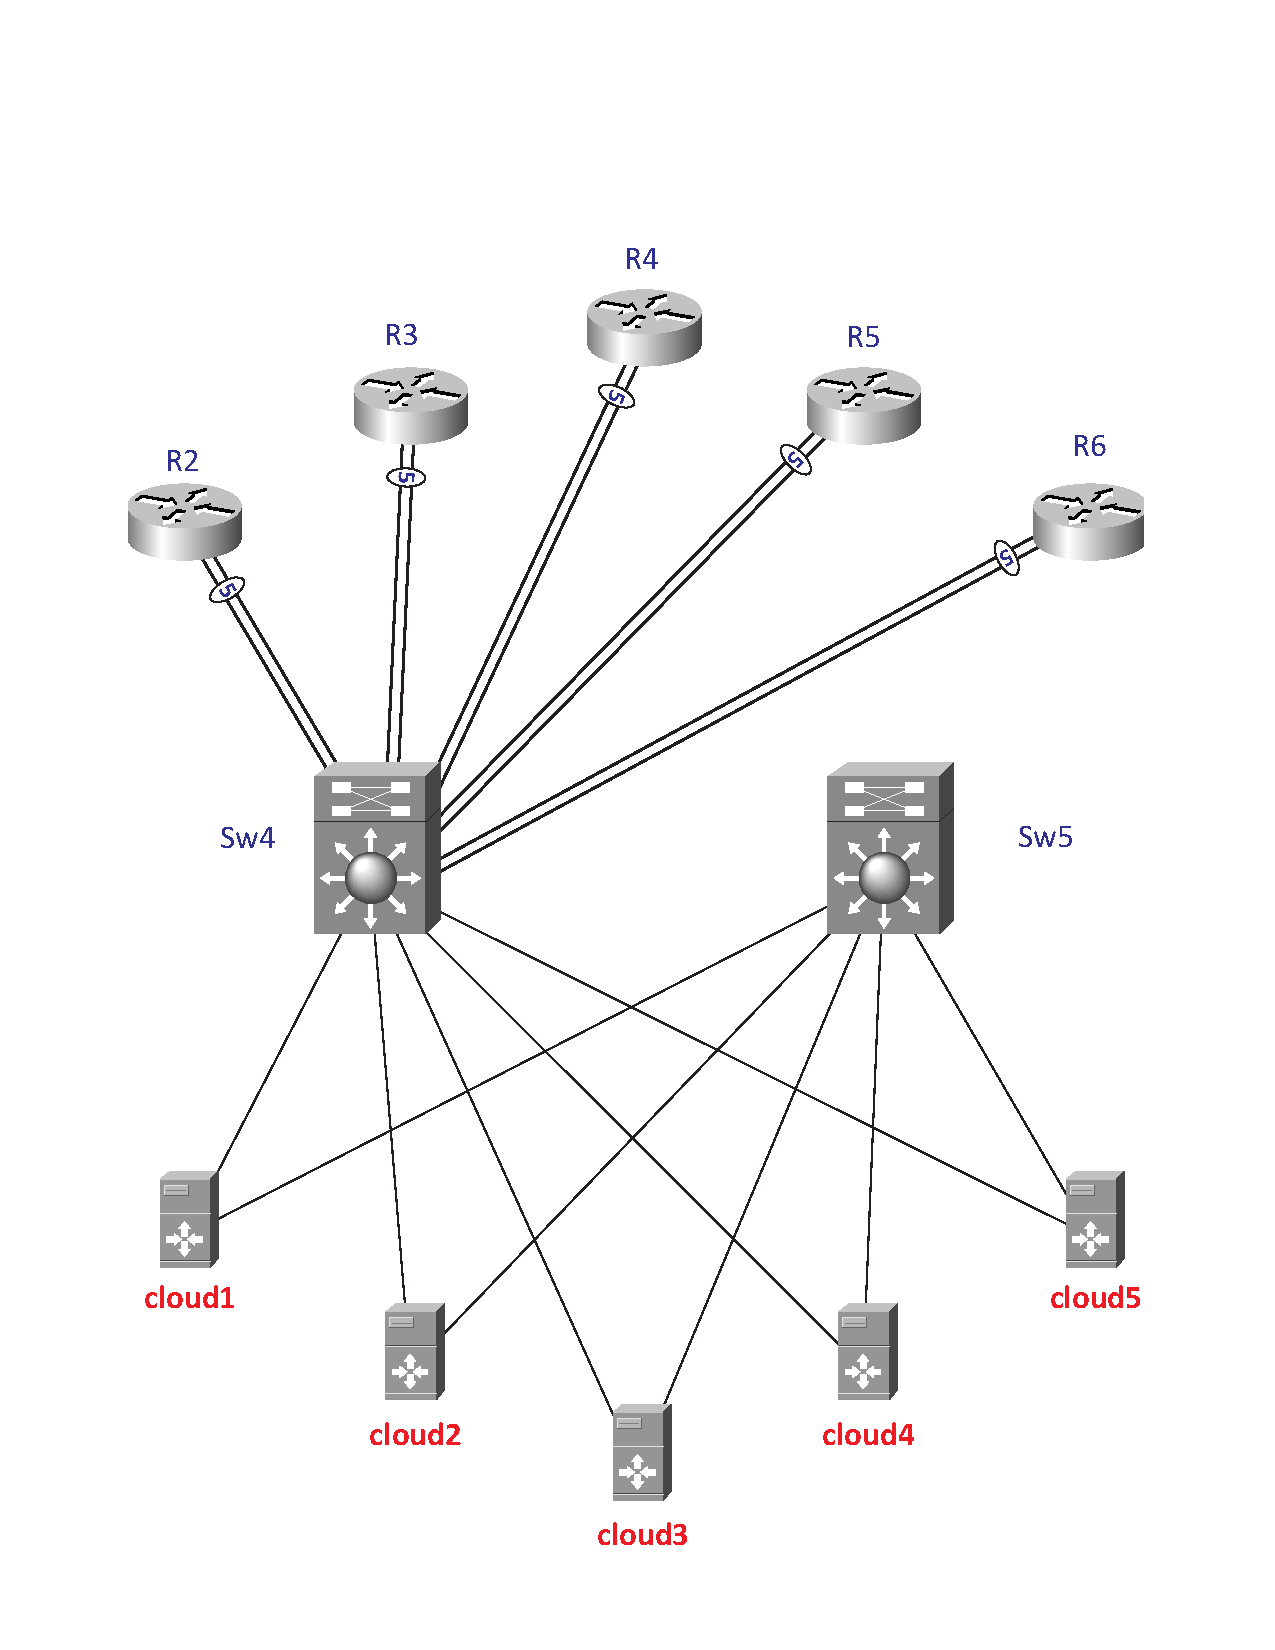
\includegraphics[width=\columnwidth]{01_physical_topology_v2_abstr}
	\caption{Physical Topology}
	\label{fig:deployment}
\end{figure}

\begin{figure}
	\centering
		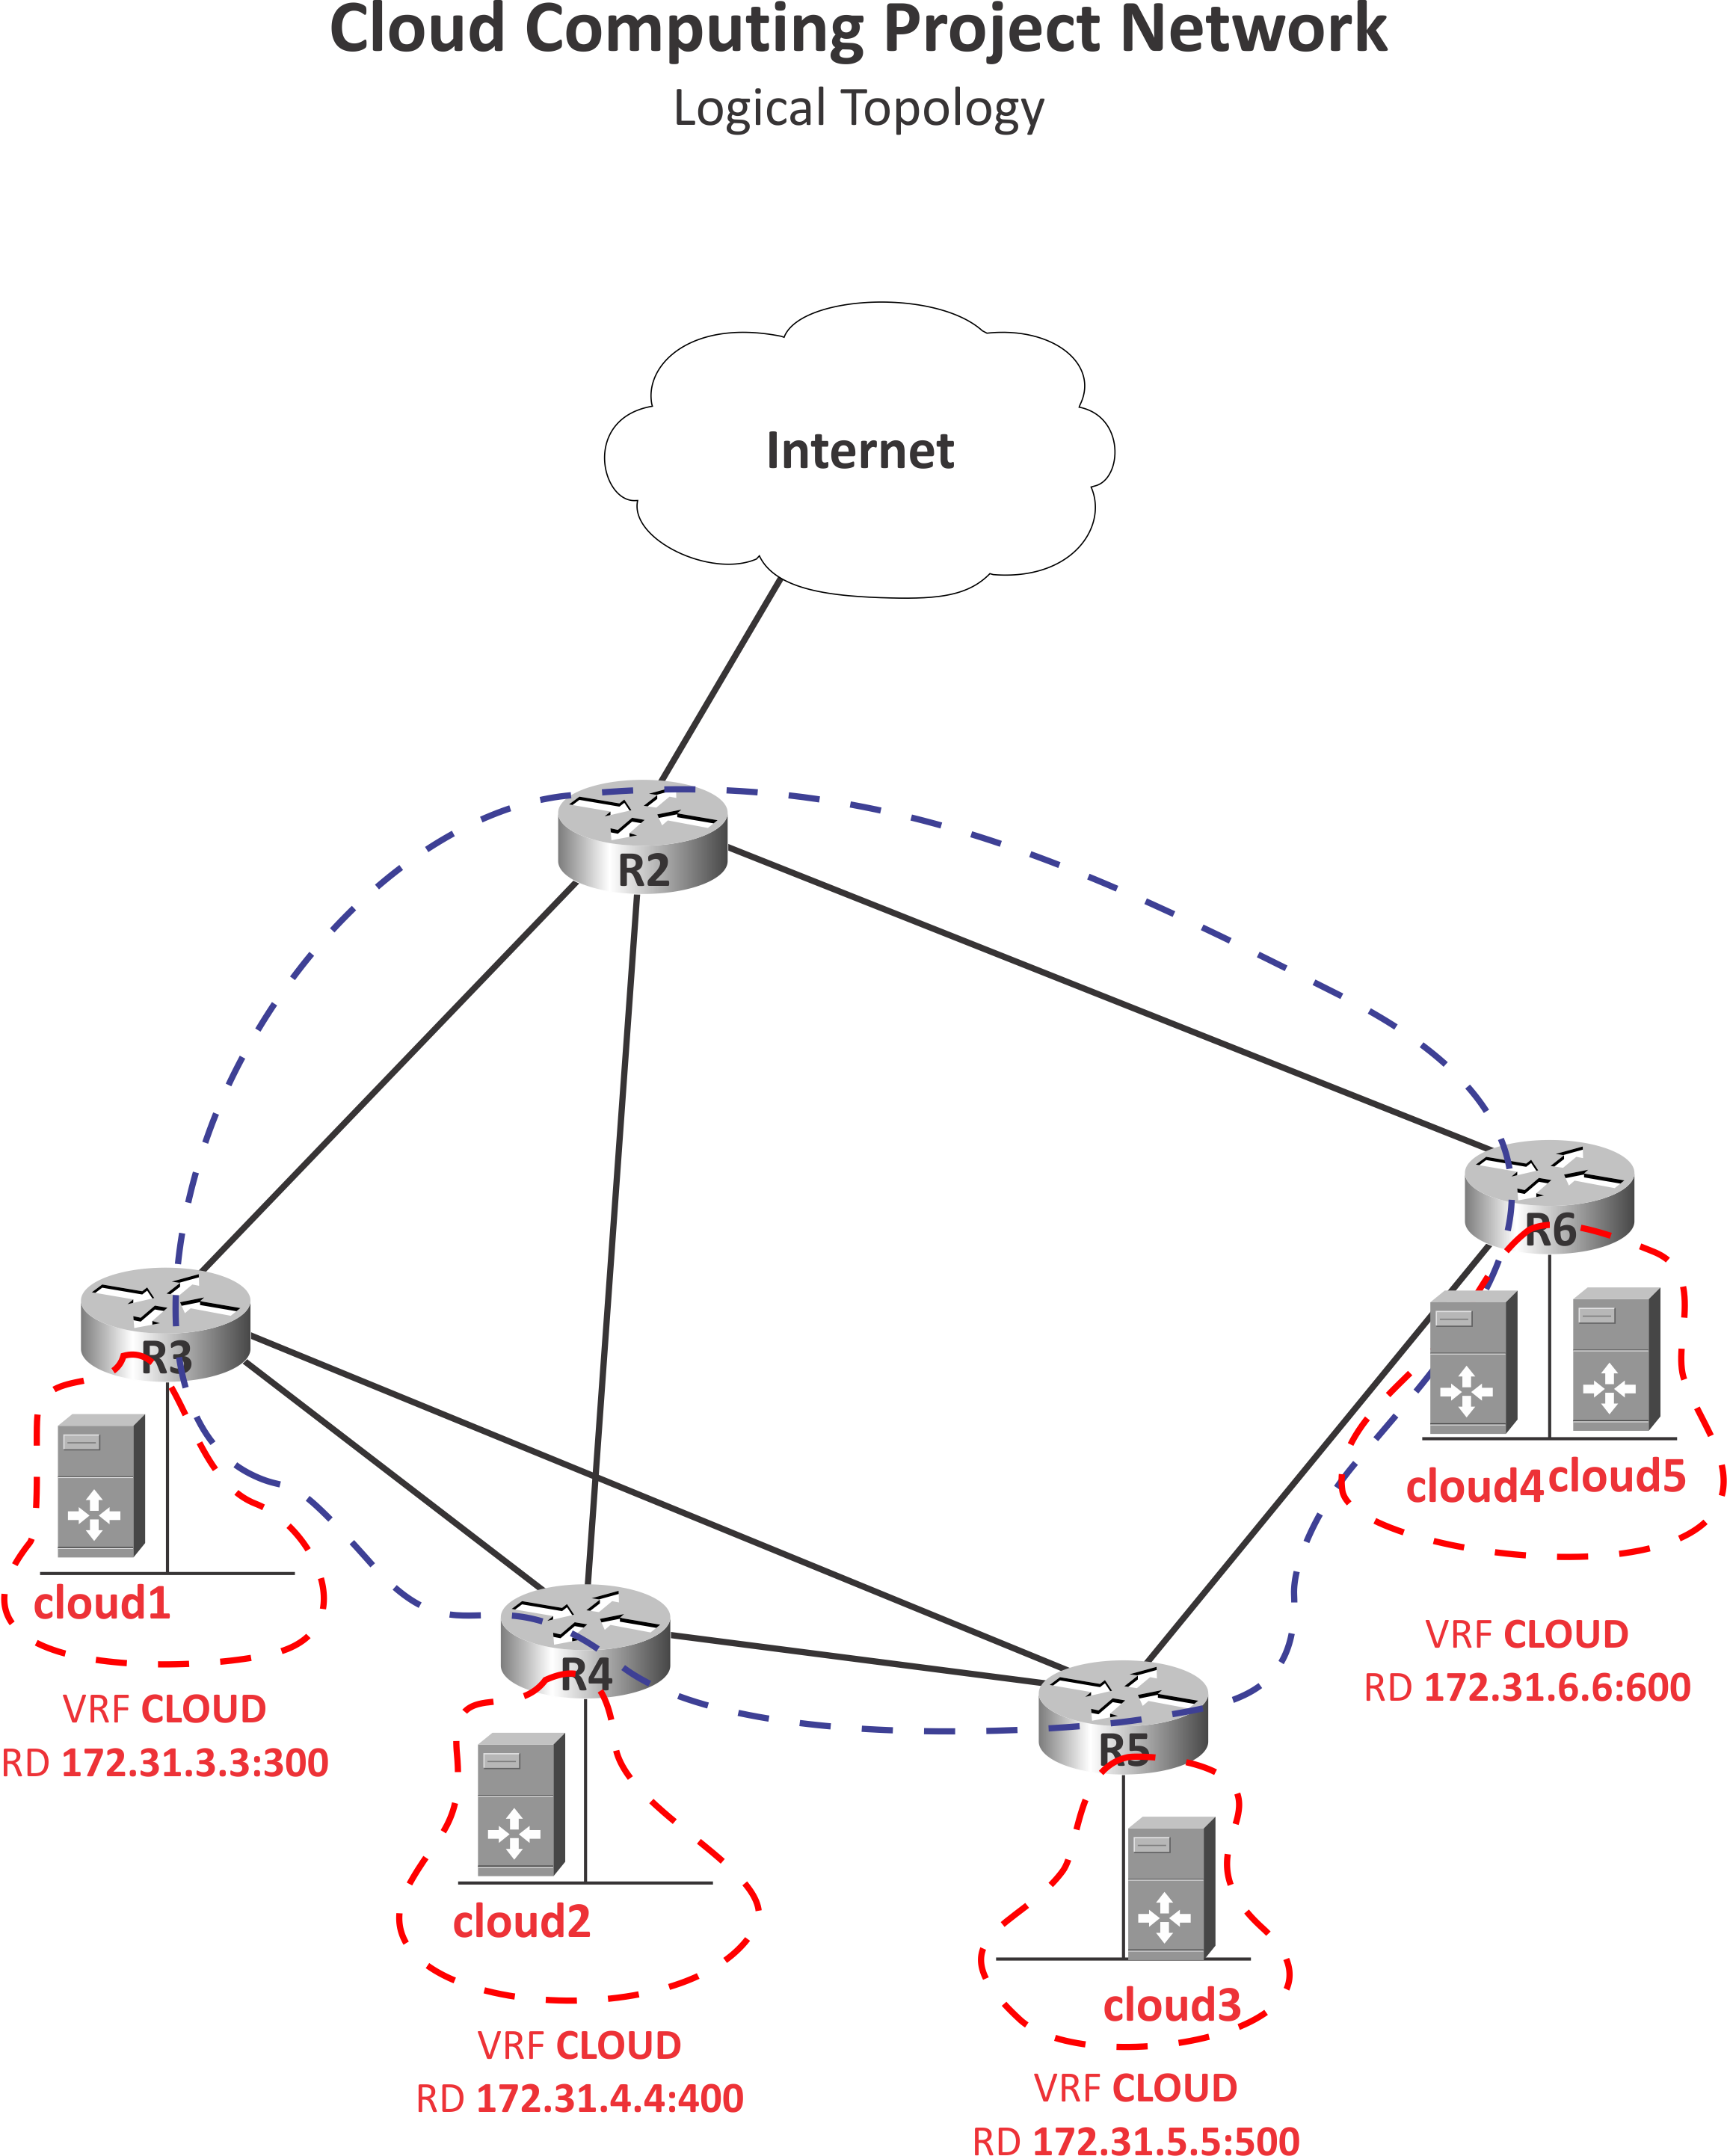
\includegraphics[width=\columnwidth]{05_logical_topology_routing_protocols_v2_abstr}
	\caption{Logical Topology Routing}
	\label{fig:logicaldeploymentrouting}
\end{figure}

A separate machine not shown in the diagrams is responsible for simulating client requests. In order to test audio/video streaming a prerecorded webcam video is streamed whenever the client simulator decides to start streaming. The stream used for testing is a 64x64 video stream at 25 frames per second with a bit rate of 180Kbps. The client simulator is written in Java and can simulate various client distributions by varying the amount of clients, the number of clients in every session, the number of clients streaming in each session and the time delay between messages being sent in a session. The simulator initially creates a number of sessions and a number of clients in each session. Each client is created with a given time to live. Periodically, the session calculates how many clients should be streaming in the session at that point in time. If more clients are required to stream than are currently streaming, the session simulator instructs a number of clients to start streaming also. If less clients are required to stream than are currently streaming, the session simulator instructs a number of clients to stop streaming. If there is no change in the number of clients needed to stream, then no change is made in which clients are streaming. Whenever a client reaches its time to live, the client is put to sleep and given a time after which it should wake up and reactivate. When a client reactivates it joins again the same session it was a member of, before going to sleep. The amount of time clients are awake and sleep is randomized thus generating various session sizes over time.

\subsection{System Behaviour Measurements}

First of all, using the test bed a number of runs were performed in order to determine the behaviour of the collaborative cloud. The tests vary one of four variables in order to determine how they affect the outputs of the media server clouds. For each of the tests presented in the following subsections one variable was modified while all others were kept constant. The four variables are the following:

\begin{enumerate}
	\item Number of servers in the cloud, varied from one to three.
	\item Number of collaborative sessions in each server, varied from one to six.
	\item Number of clients in each session, varied in increments of one from two to forty. In some cases, the increases in clients stopped before reaching the maximum due to the 10Mbps network link becoming saturated.
	\item Number of clients streaming per session, varied from one to four. 
\end{enumerate}

The tests presented here represent an exhaustive search of the variable space in order to determine how each of the four variables affects the system under test.

\subsection{Test Plan}

The data is measured from all the servers every 30 seconds, and is composed of: bandwidth received, bandwidth sent, latency and CPU usage. Since the tests are run at different moments in time, the timescale is normalized to the period from when each test was started.

The expectations are that as the number of servers increases for a given number of clients, sessions and streams the bandwidth and latency will decrease proportionally. Similar, as the number of collaborative sessions increases, with all other variables kept constant bandwidth and latency will decrease as the 1:N proportion, where N is how many clients receive the stream decreases. When the number of clients in a session increases bandwidth and latency should increase in a reverse fashion. Finally, when the number of streaming clients increases bandwidth and latency should increase similarly.

The graphs for the performance tests can be found online as they would take too much space here. In order to make the results more visible, the tests are grouped on the graphs 3 by 3, with the lowest test on one graph being the highest test on another graph. The following sections will present some of the results in tabular form and the rest of the results can be found online as well.

In order to simplify notations, test will be abbreviated in the form servers/sessions/incoming streams per session. For example, the test 3/1/4refers to a test with 3 servers, 1 session across all servers and 4 incoming streams from clients.

\subsubsection{1 Server, 1 Collaborative Session, 1 Stream Per Session}
\label{sec:1serv_1sess_1str}

The number of clients was varied from 2 to 40 in increments of 1. The number of outgoing streams is equal to (the number of users - 1) because the streaming user does not receive the stream back. These results show that as the number of users increases in a session, the latencies and CPU usage of the server increase at the same time. Interestingly mean CPU usage seems to reach an upper bound around 34 users while latencies continue to increase.

\subsubsection{1 Server, 1 Collaborative Session, 2 Streams Per Session}
\label{sec:1serv_1sess_2str180}

The number of clients was varied from 2 to 20 in increments of 1. The number of outgoing streams in this case will be equal to 2 * (the number of users - 1), as there are 2 streams going to all users in the session except the streamer. The pattern is similar to the previous case, with latencies and CPU usage increasing as the number of users in the session increases. Similar to before, CPU reaches a point where it peaks while latencies still increase. If similar numbers of outgoing streams were to be compared, it can be seen that the results are similar in both CPU usage and latency at lower number of users. For example, for 12 outgoing streams the previous test had a median CPU of 19.28 \% and median latency of 15.69 ms, while this test has a median CPU of 19.35 \% and median latency of 16.71ms. As the number of users increases however, the results of this test case are worse than the equivalent result of the previous test. For example, for 26 outgoing streams the previous test had a median CPU of 36.09 \% and median latency of 20.63 ms, while this test has a median CPU of 31.06 \% and median latency of 22.64 ms.

\subsubsection{1 Server, 1 Collaborative Session, 3 Streams Per Session}
\label{sec:1serv_1sess_3str180}

The number of clients was varied from 3 to 14 in increments of 1. The number of outgoing streams in this case will be equal to 3 * (the number of users - 1), as there are 3 streams going to all users in the session except the streamer. Like in the two previous cases CPU and latency increase as more users are added to the session. At similar levels of outgoing streams, the results for this test case are a bit worse than those of the two previous tests. For 12 outgoing streams, this results in a median latency of 20.41 ms, which is higher than 16.71 ms for the previous test and 15.69 ms for the first test.

\begin{table}
\caption{Median and Mean CPU, Latencies for 1 Server, 1 Session, 3 Stream}
\label{table:1serv_1sess_3str}
\begin{tabu} to\linewidth{|X[c]|X[c]|X[c]|X[c]|X[c]|X[c]|X[c]|X[c]|}
\everyrow{\hline}
\hline
Nr. of Users & Median Latency (ms) & Mean Latency (ms) & Median Message Latency (ms) & Mean Message Latency (ms) & Median CPU (\%) & Mean CPU (\%) & Out Stream Count\\
\taburowcolors 2{Gray!20..LimeGreen!50}
3 & 11.83 & 26.84 & 10 & 159.44 & 12.2 & 10.36 & 6 \\
4 & 11.75 & 23.48 & 10 & 22.25 & 16.49 & 14.38 & 9 \\
5 & 13.2 & 28.18 & 9 & 139.88 & 20.41 & 16.79 & 12 \\
6 & 17 & 22.06 & 10 & 53.82 & 20.04 & 16.42 & 15 \\
7 & 17.43 & 24.73 & 10 & 17.33 & 22.94 & 19.22 & 18 \\
8 & 16.25 & 28.08 & 10 & 32.48 & 26.24 & 22.29 & 21 \\
9 & 20.11 & 43.52 & 10 & 25.36 & 31.03 & 26.28 & 24 \\
10 & 19.3 & 31.01 & 11 & 53.42 & 34.48 & 29.43 & 27 \\
11 & 25.73 & 75.89 & 15 & 46.64 & 32.74 & 27.37 & 30 \\
12 & 30 & 67.83 & 15 & 45.34 & 35.04 & 29.77 & 33 \\
13 & 45.08 & 99.52 & 32 & 53.17 & 36.2 & 30.95 & 36 \\
14 & 76.82 & 112.76 & 34 & 39.84 & 39.52 & 34.06 & 39 \\
\end{tabu}
\end{table}

\subsubsection{1 Server, 1 Collaborative Session, 4 Streams Per Session}
\label{sec:1serv_1sess_4str180}

For this test, users were varied from 4 to 11 in increments of 1. Outgoing streams behave as previous and will be equal to 4 * (the number of outgoing streams). Same results as for the previous tests are observed, as median latency for 12 outgoing streams is even higher than the previous tests.

\begin{table}
\caption{Median and Mean CPU, Latencies for 1 Server, 1 Session, 4 Stream}
\label{table:1serv_1sess_4str}
\begin{tabu} to\linewidth{|X[c]|X[c]|X[c]|X[c]|X[c]|X[c]|X[c]|X[c]|}
\everyrow{\hline}
\hline
Nr. of Users & Median Latency (ms) & Mean Latency (ms) & Median Message Latency (ms) & Mean Message Latency (ms) & Median CPU (\%) & Mean CPU (\%) & Out Stream Count\\
\taburowcolors 2{Gray!20..LimeGreen!50}
4 & 11.88 & 17.23 & 10 & 14.55 & 21.59 & 18.1 & 12 \\
5 & 14.2 & 20.44 & 10 & 38.31 & 21.88 & 18.22 & 16 \\
6 & 18.33 & 26.47 & 11 & 37.45 & 27.19 & 22.72 & 20 \\
7 & 20.14 & 39.64 & 11.5 & 32.15 & 33.14 & 27.96 & 24 \\
8 & 22.62 & 49.37 & 13 & 26.71 & 35.71 & 30.28 & 28 \\
9 & 32.89 & 79.52 & 20.5 & 34.98 & 35.84 & 29.86 & 32 \\
10 & 30 & 82.61 & 24.5 & 54.45 & 37.32 & 31.55 & 36 \\
11 & 69.45 & 107.49 & 40 & 45.13 & 38.35 & 32.62 & 40 \\
\end{tabu}
\end{table}

\subsubsection{1 Server, 2 Collaborative Sessions, 1 Stream}
\label{sec:1serv_2sess_1str180}

In this test 2 collaborative sessions of equal size are created, but only one session contains a streaming client. In the second session, clients only exchange text/synchronization messages. The goal of this test is to determine if there are other factors in the application outside video/audio streaming impacting latencies and CPU usage. If this test was compared to the test in section \ref{sec:1serv_1sess_1str}, it would be expected that latencies are very similar for equal numbers of clients. This expectation is not met however, as similar numbers of users result in higher latencies for this test. CPU usage values are very close for all tests however. This suggests that first of all, latencies are not directly related to CPU usage, and at the same time that only the number of outgoing streams is not sufficient to determine the latency of the system.

\subsubsection{1 Server, 2 Collaborative Sessions, 4 Streams}
\label{sec:1serv_2sess_4str}

The same trend as before is shown by this test when compared to both the previous tests with 2 sessions and to the 1/1/4 test.

\begin{table}
\caption{Median and Mean CPU, Latencies for 1 Server, 2 Session, 4 Stream}
\label{table:1serv_2sess_4str}
\begin{tabu} to\linewidth{|X[c]|X[c]|X[c]|X[c]|X[c]|X[c]|X[c]|X[c]|}
\everyrow{\hline}
\hline
Nr. of Users/Session & Median Latency (ms) & Mean Latency (ms) & Median Message Latency (ms) & Mean Message Latency (ms) & Median CPU (\%) & Mean CPU (\%) & Out Stream Count\\
\taburowcolors 2{Gray!20..LimeGreen!50}
2 & 12.25 & 16.02 & 12 & 58.94 & 10.91 & 9.42 & 4 \\
3 & 16 & 24.18 & 12 & 20.44 & 16.75 & 13.7 & 8 \\
4 & 16.69 & 23.48 & 12 & 17.18 & 21.78 & 18.28 & 12 \\
5 & 16.25 & 27.37 & 11 & 52.32 & 22.55 & 19.18 & 16 \\
6 & 19.17 & 31.97 & 12 & 30.2 & 28.5 & 23.87 & 20 \\
7 & 22.79 & 49.1 & 12.5 & 33.83 & 31.85 & 26.27 & 24 \\
8 & 27.38 & 77.3 & 12.5 & 26.23 & 37.85 & 32.18 & 28 \\
9 & 45 & 77.44 & 20 & 35.24 & 36.82 & 31.38 & 32 \\
10 & 71.6 & 116.25 & 21 & 35.18 & 38.2 & 32.99 & 36 \\
\end{tabu}
\end{table}

\subsubsection{1 Server, 3 Collaborative Sessions, 3 Streams}
\label{sec:1serv_3sess_3str}

Comparing this test results with the results for 1 Server, 2 Collaborative Sessions, 3 Streams, for the same number of outgoing streams, CPU usage is very similar, while latencies are higher for this test. The reason for this, is that a similar number of outgoing streams for this case has more total users across the server.

\begin{table}
\caption{Median and Mean CPU, Latencies for 1 Server, 3 Session, 3 Stream}
\label{table:1serv_3sess_3str}
\begin{tabu} to\linewidth{|X[c]|X[c]|X[c]|X[c]|X[c]|X[c]|X[c]|X[c]|}
\everyrow{\hline}
\hline
Nr. of Users/Session & Median Latency (ms) & Mean Latency (ms) & Median Message Latency (ms) & Mean Message Latency (ms) & Median CPU (\%) & Mean CPU (\%) & Out Stream Count\\
\taburowcolors 2{Gray!20..LimeGreen!50}
2 & 14 & 19.06 & 11 & 16.43 & 8.3 & 7.43 & 3 \\
3 & 13.56 & 17.83 & 11 & 40.74 & 12.6 & 10.84 & 6 \\
4 & 16.17 & 18.44 & 11 & 28.72 & 16.86 & 14.9 & 9 \\
5 & 16.33 & 28.52 & 10 & 15.91 & 20.82 & 18.06 & 12 \\
6 & 19.89 & 28.45 & 11 & 18.02 & 20.84 & 17.52 & 15 \\
7 & 22.81 & 34.21 & 11 & 18.98 & 23.46 & 19.77 & 18 \\
8 & 20.9 & 38.72 & 11 & 21.45 & 29.21 & 24.71 & 21 \\
9 & 27.81 & 40.85 & 11 & 22.38 & 33.17 & 27.21 & 24 \\
10 & 35.65 & 73.61 & 11 & 26.09 & 35.04 & 29.64 & 27 \\
11 & 44.55 & 82.58 & 14.5 & 33.29 & 35.46 & 30.34 & 30 \\
12 & 40.06 & 111.62 & 15 & 31.79 & 38.11 & 31.4 & 33 \\
13 & 107.77 & 134.55 & 27.5 & 40.45 & 39 & 32.78 & 36 \\
14 & 71.73 & 126.28 & 18 & 31.79 & 39.02 & 28.9 & 39 \\
\end{tabu}
\end{table}

\subsubsection{2 Servers, 1 Collaborative Session, 3 Streams}

Comparing this test with the test for 1 Servers, 1 Collaborative Session, 3 Streams, the latency and CPU usage are similar for an equal number of outgoing streams. Doing the same comparison with the test for for 1 Server, 2 Collaborative Sessions, 3 Streams, the results are better for this result.

\begin{table}
\caption{Median and Mean CPU, Latencies for 2 Server, 1 Session, 3 Stream}
\label{table:2serv_1sess_3str}
\begin{tabu} to\linewidth{|X[c]|X[c]|X[c]|X[c]|X[c]|X[c]|X[c]|X[c]|}
\everyrow{\hline}
\hline
Nr. of Users/Server & Median Latency (ms) & Mean Latency (ms) & Median Message Latency (ms) & Mean Message Latency (ms) & Median CPU (\%) & Mean CPU (\%) & Out Stream Count\\
\taburowcolors 2{Gray!20..LimeGreen!50}
2 & 11 & 30.57 & 33 & 25.02 & 10.34 & 8.61 & 6 \\
3 & 14.33 & 22.17 & 32 & 24.33 & 13.46 & 11.44 & 9 \\
4 & 14.38 & 29.36 & 33.5 & 198.07 & 16.97 & 14.19 & 12 \\
5 & 15.2 & 20.99 & 35 & 86.81 & 19.98 & 16.18 & 15 \\
6 & 15.67 & 18.74 & 35 & 48.21 & 23.45 & 19.46 & 18 \\
7 & 19.14 & 36.61 & 36 & 33.92 & 26.53 & 22.04 & 21 \\
8 & 16.38 & 30.7 & 36 & 34.27 & 30.44 & 25.37 & 24 \\
9 & 19.22 & 38.75 & 37 & 39.36 & 33.24 & 26.62 & 27 \\
10 & 25.2 & 46 & 40.5 & 43.95 & 35.07 & 28.68 & 30 \\
11 & 21.45 & 59.71 & 45.5 & 104.72 & 36.31 & 29.23 & 33 \\
12 & 36 & 68.65 & 44 & 52.64 & 38.89 & 31.28 & 36 \\
13 & 62.77 & 91.37 & 60.5 & 69.6 & 40.33 & 33.35 & 39 \\
\end{tabu}
\end{table}

\subsubsection{2 Servers, 3 Collaborative Sessions, 6 Streams}

Comparing results between this test and the test for 1 server, 3 sessions and 6 streams, median latency is better for this test while CPU results are similar for equal number of outgoing streams.
 
\begin{table}
\caption{Median and Mean CPU, Latencies for 2 Server, 3 Session, 6 Stream}
\label{table:2serv_3sess_6str}
\begin{tabu} to\linewidth{|X[c]|X[c]|X[c]|X[c]|X[c]|X[c]|X[c]|X[c]|}
\everyrow{\hline}
\hline
Nr. of Users per Session per Server & Median Latency (ms) & Mean Latency (ms) & Median Message Latency (ms) & Mean Message Latency (ms) & Median CPU (\%) & Mean CPU (\%) & Out Stream Count\\
\taburowcolors 2{Gray!20..LimeGreen!50}
1 & 13.67 & 27.24 & 38 & 112.94 & 13.02 & 11.24 & 6 \\
2 & 16.67 & 39.36 & 35 & 43.1 & 20.53 & 17.69 & 12 \\
3 & 15.56 & 23.39 & 38 & 59.07 & 27.73 & 24.17 & 18 \\
4 & 20.17 & 25.18 & 37 & 71.53 & 32.97 & 28.19 & 24 \\
5 & 20.93 & 52.74 & 32 & 45.75 & 35.89 & 31.04 & 30 \\
6 & 44.11 & 73.98 & 46.5 & 49.17 & 37.99 & 33.04 & 36 \\
\end{tabu}
\end{table}

\subsubsection{Test Conclusions and Identification}

The tests presented in the previous sections can be compared in a number of ways. The first way to compare them is to look at tests with a similar number of incoming streams and sessions. For example, looking at tests with 1 session and 1 client streaming, it can be noticed that the median latency and median CPU usage are close to each other for all tests for similar numbers of clients connected. Tests 1/1/1, 2/1/1, and 2/2/1/1 all show similar results for 10, 20, 30 and 36 users. At the same time tests 1/2/1 and 2/2/1 have similar results to each other, but have higher median latencies and similar CPU usage at 10, 20, 30 and 36 users compared to the tests with 1 session. This is most likely due to having more users connected. The same behaviour can be noticed for the tests with 2 clients streaming.

Another way to compare the tests results is by looking at results with the same number of collaboration sessions. By comparing these results it can be observed that as the number of incoming streams increases, latency decreases, while CPU is the same across the tests. For the same number of outgoing streams - tests 1/1/1, 1/1/2, 1/1/3 and 1/1/4 for example - it can be seen that results from 1 incoming streams are better than results for 4 incoming streams when there is the same number of outgoing streams. This can be explained by the fact that in order for the test to have the same number of outgoing streams, as the incoming stream count increases less users are in a session. The same behaviour can be observed across the other tests with equal number of sessions.

Looking at tests with the same number of sessions and streams but different numbers of servers, it can be noticed that the results are the same across different tests if the only variable is the number of servers. Similar behaviour can be observed if the only variable is the number of clouds, with everything else being constant. This confirms the assumption that better performance can be obtained by spreading the users across multiple servers.

If tests with similar numbers of outgoing streams are compared, it can be noticed that as the number of total users connected to each of the servers increases, the performance decreases. This however, does not apply just based on number of users connected. For example, comparing the results of tests with 30 outgoing streams, the worst result is shown by the 1/2/1 test which also has the most users connected (62 users), while the best result is shown by the test 1/1/2 which has 16 users connected. Tests for 1/1/1, 1/2/2 and 1/3/3, have similar numbers of users connected - 31 users, 32 users and 33 users respectively. However, 1/1/1 has much better results than 1/2/2 which has better results than 1/3/3. This could be explained by the fact that the tests with worse results have more incoming streams.

As such, it can be assumed that median latency is a function of number of users connected, and the number of incoming streams. This information is used in order to build a fuzzy system to control the cloud of collaborative servers.

\subsection{Collaborative cloud control system}

For the purpose of controlling the collaborative cloud, each server has its own control loop, similar to the one developed in \cite{bogdan:seams07}. The architecture can be seen in Figure \ref{fig:selfopt-archi}.

\begin{figure}
	\centering
	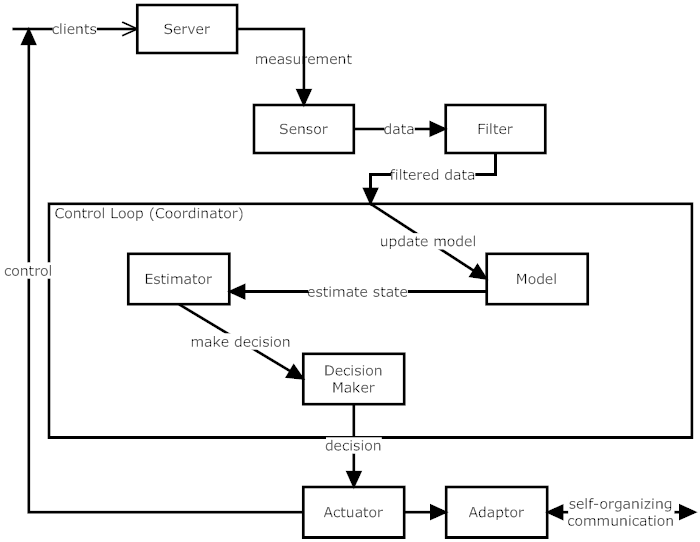
\includegraphics[width=0.9\linewidth]{Self-optimizingControlLoop_full}
	\caption{Self-Optimizing Control Loop Architecture}
	\label{fig:selfopt-archi}
\end{figure}

Each collaborative server can be seen as having one perturbation signal which is the arrival of requests from clients connected to the server. Some requests, like video streaming, are more demanding on the server than others. As requests are processed, the CPU usage and response time of the server will change. More requests or more demanding requests will lead to higher CPU usage and an increase in response time. As the number of requests decreases, the CPU usage and response time will also decrease. Based on the measured sensor data, the control loop uses a fuzzy model and estimator to predict the response time for the next sampling period. This prediction is used in order to decide if the server should accept connections or not. The block diagram can be mapped to the eight component based architecture through the following steps:

\begin{enumerate}
	\item Implement a sensor which measures the desired data from the media server. The measured data includes:
	\begin{enumerate}
		\item CPU usage
		\item Number of connected clients
		\item Number of collaborative rooms
		\item Number of clients connected to all media servers in the cloud
		\item Network latency
		\item Bandwidth up/down
		\item Number of streams incoming/outgoing from server
	\end{enumerate}
	\item Add a filter which computes the numbers of packets in and out from the bandwidth up/down
	\item Add a fuzzy model which calculates the confidence that the server is overloaded. The fuzzy model computes two fuzzy functions:
	\begin{enumerate}
		\item Compute confidence1 based on number of clients, packets out, packets in and number of incoming streams.
		\item Compute confidence2 based on packets in and CPU usage
		\item Take the maximum value of the two confidences
	\end{enumerate}
	\item Add an estimator which compares the confidence from the model with two given thresholds. If the confidence is above the higher threshold increment a counter of how many times the system was above the higher threshold. Similarly if the confidence is bellow the threshold increment a counter of how many time the system was bellow the lower threshold.
	\item Add a decision maker which uses the count of how many times the system was above/bellow the thresholds in the estimator to decide if the server should accept or reject connections. If the server is above the higher threshold for more than a given count, then the server stops accepting new clients. If the server is bellow the lower threshold for a given amount of time and is not accepting clients, then it starts accepting clients.
	\item Add an actuator which communicates with the cloud load balancer. If the server should not accept connections then the actuator sends a message to the load balancer that it should stop redirecting new clients to it. Conversely, if the server should start accepting clients again, then it sends a message that the load balancer can start redirecting clients to it.
	\item The coordinator simply coordinates the control loop and passes messages between model, controller, decision maker and actuator.
\end{enumerate}

The control system for each media server is an application separated from the media server and deployed in a separate container from the media server. It can connect to the media server to retrieve sensor data but has no other interactions with the media server. The control system can also act on behalf of the media server to ask the load balancer to redirect or stop redirecting new clients to the media server. The overall control architecture looks as Figure \ref{fig:control-containers}

\begin{figure}
	\centering
	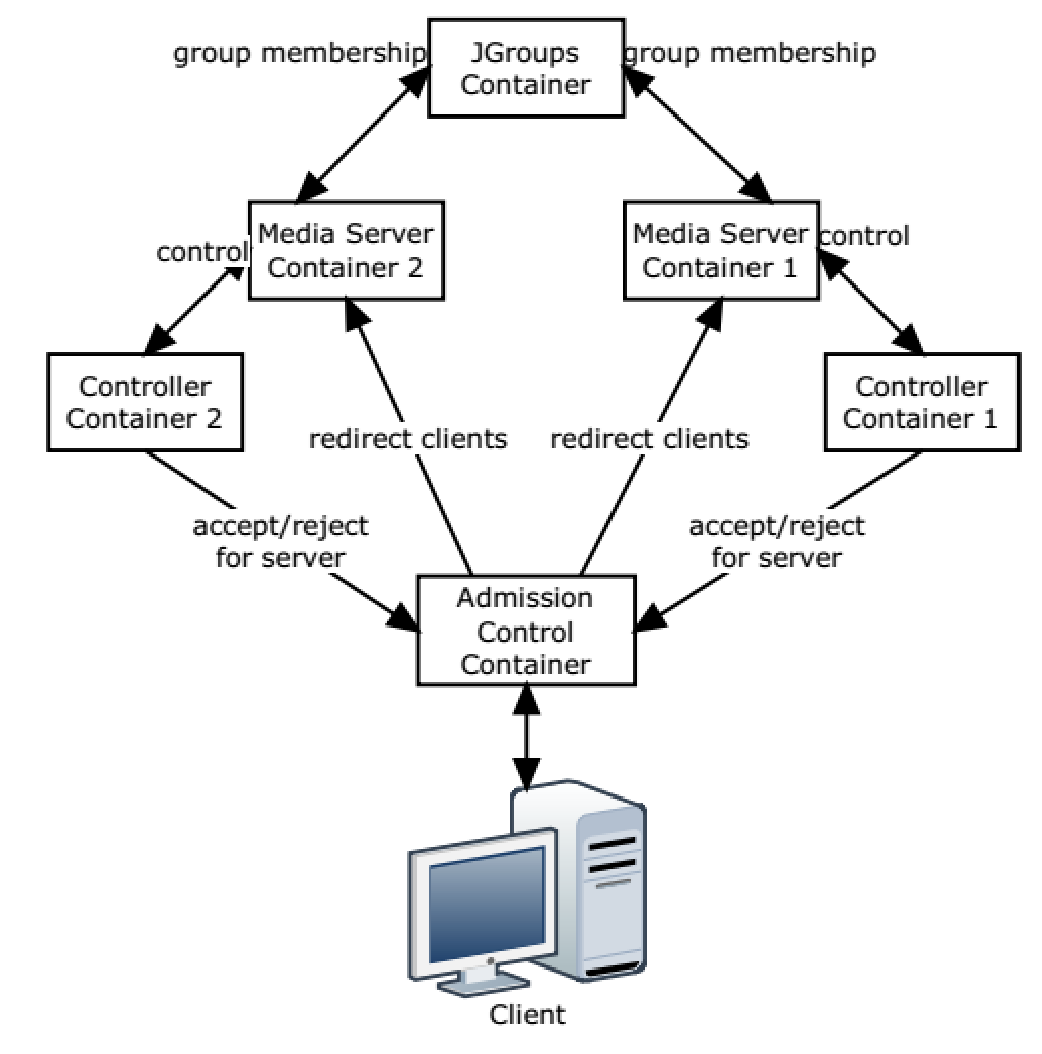
\includegraphics[width=0.9\linewidth]{containers_control}
	\caption{Control System}
	\label{fig:control-containers}
\end{figure}

The results of the fuzzy control system are also fed as an input to the ACO algorithm in order to predict when an SLA breach will happen and serves need to be added or removed from the cloud.

\section{Simulation environment}

The second set of performance tests for the self-organizing management of cloud resources presented in this thesis was a simulation developed on top of the CloudSim and CloudSimEx systems. CloudSim is a framework for modelling and simulating cloud systems in which various tests can be run - for example the placement of tasks in a cloud or the performance of a cloud system. CloudSim allows users to define datacenters which are composed of hosts which can run virtual machines and virtual machines which run on top of the hosts. Both hosts and virtual machines are defined in terms of million instructions per second (MIPS) and memory available. Once a datacenter is defined, a workload can be defined as well to be executed in the datacenter. CloudSim workloads are called cloudlets - a cloudlet represents a user task and defines how many million instructions (MI) the task takes as well as how much memory the task needs. As such a cloudlet's execution time will depend on its' lifetime in MIs and how many MIPS the VM the cloudlet is allocated to has. The usage of MIPS and MI to represent loads and available resources make it complicated to define workloads that would represent real world behaviours.

CloudSimEx extends CloudSim by adding the concept of web sessions. Internally a web session is composed of a number of web cloudlets, where each web cloudlet has a small RAM and MIPS requirements and later web cloudlets in a web session can not be completed until all previous web cloudlets have completed. Web sessions also have the property of targeting both application server VMs and database VMs, with the web session alternating cloudlets running on either application server or database server. Furthermore, CloudSimEx also adds the concept of scaling policies which can be applied on a cloud. A scaling policy adds or removes servers to/from the cloud when the policy determines that some conditions are breached. A basic policy is implemented in CloudSimEx which scales the cloud when the CPU usage passes certain thresholds and also includes a quiet time after a scaling action has been performed. The basic policy implements an interface which makes it easy to add other scaling policies. 

Because CloudSim and CloudSimEx only include CPU usage and memory usage as measurable metrics, the simulation of the self-organizing system uses the CPU usage as an input for the ACO algorithm to determine how the pheromone should be updated. In order to run the self-organizing system in this thesis and compare it to existing results, a number of workloads which are predefined in CloudSimEx are used.

The architecture of the simulation framework is presented in Figure \ref{fig:simulation-design}.


\begin{figure}
	\centering
	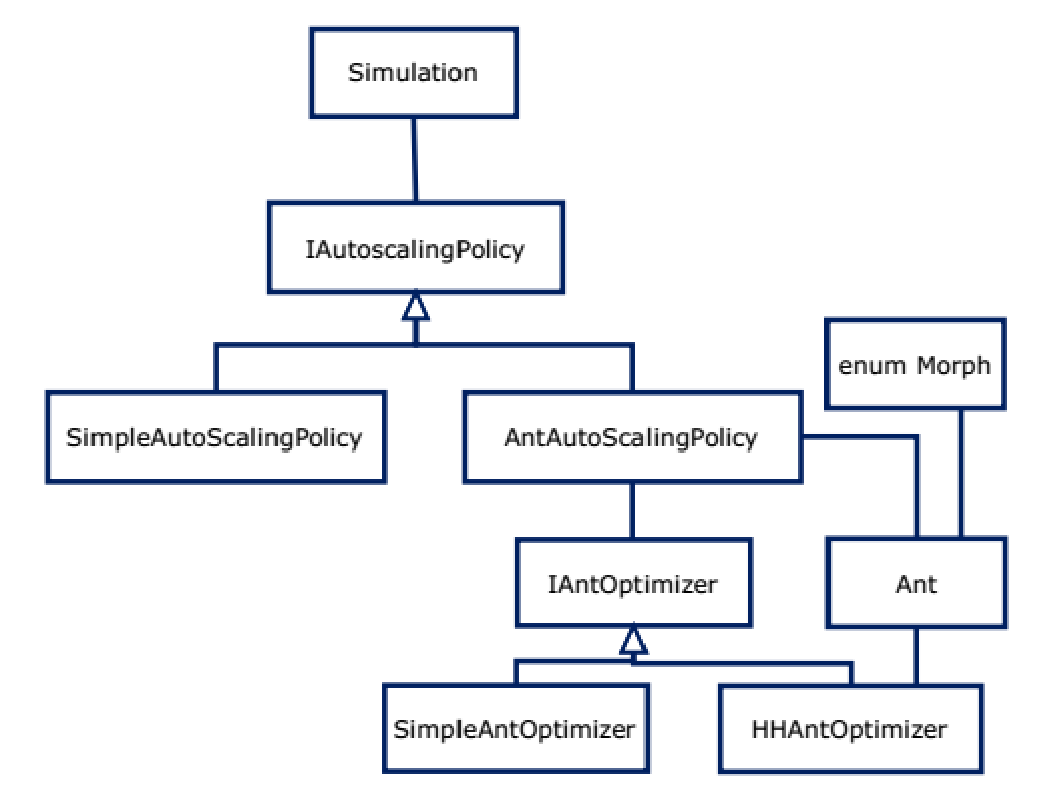
\includegraphics[width=0.9\linewidth]{simulation_archi}
	\caption{Simulation Framework System}
	\label{fig:simulation-design}
\end{figure}

%description of diagram

The simulation runs three different scaling policies for comparison. The first scaling policy used is the simple scaling policy provided by CloudSimEx. This scaling policy measures the average CPU usage of the cloud and when predefined thresholds are breached it either adds one server if the upper threshold is breached or removes one server if the lower threshold is breached. The policy also includes a quiet time, which is a period of time after an action was taken during which no other action will be taken. For the purpose of these tests the thresholds for the simple scaling policy are set to:

\begin{description}
	\item[Upper threshold] is set to 80\% average CPU utilization across the cloud
	\item[Lower threshold] is set to 10\% average CPU utilization across the cloud
	\item[Quiet time] is set to 150s during which no other action will be taken
\end{description}

The values chosen match the default values for the Amazon EC2 auto scaling policy.

The second policy is based on the predictive ACO algorithm presented in this thesis but without the house hunting algorithm to determine the number of instances to scale up or down. The policy uses the ACO algorithm to determine when instances should be added or removed. When a decision is taken that servers need to be added or removed a single server instance is added or removed at one time. The ACO policy does not need quiet time defined as it inherently includes quiet time due to the fact that it takes time for the pheromone to build up or decrease. For the purpose of these simulations the ACO algorithm runs with the following parameters:

\begin{description}
	\item[Decay amount] is set to 1
	\item[Decay period] is set to 15s
	\item[Minimum ant wait time at an under-loaded node] is set to 1s
	\item[Maximum ant pheromone added at an under-loaded node] is set to 4
	\item[Ant memory size] is set to 5
	\item[Pheromone level for triggering server removal] is set to 100
	\item[Pheromone level for triggering server addition] is set to 25
	\item[CPU is considered to be balanced] if it is between 45\% and 55\% utilization
\end{description}

The third tested policy contains both the ACO algorithm for prediction of SLA breaches and the house hunting algorithm for the optimization of the cloud size when a breach is detected. The tests are run with the same parameters as the second policy.

Chapter \ref{Chapter_performance} will present the results for both the test-bed and the simulation.
